\documentclass[11pt]{article}

\usepackage{amsmath,amsfonts,amssymb,amsthm}
\usepackage[margin=1in]{geometry}
\usepackage[colorlinks]{hyperref}
\usepackage{algpseudocode}
\usepackage{algorithmicx}
\usepackage{listings}
\usepackage{multirow}
\usepackage{hyperref}
\usepackage{fancyhdr}
\usepackage{framed}
\usepackage{graphicx}
\usepackage{caption}
\usepackage{subcaption}
\usepackage{float}
\usepackage{enumerate}
\usepackage{tikz}
\usetikzlibrary{arrows}
\usetikzlibrary{shapes}

\newcommand{\C}{{\mathbb{C}}}
\newcommand{\F}{{\mathbb{F}}}
\newcommand{\R}{{\mathbb{R}}}
\newcommand{\Z}{{\mathbb{Z}}}
\newcommand{\e}[1]{\ensuremath{\times 10^{#1}}}

\newcommand{\ve}[1]{\boldsymbol{#1}}
\newcommand{\norm}[1]{\|{#1}\|}
\newcommand{\code}{\begingroup
	\catcode`_=12 \docode}
\newcommand{\docode}[2]{
	\begin{framed}
		\lstinputlisting[basicstyle=\ttfamily\scriptsize,language=#2,title=\underline{\texttt{#1}},tabsize=4,numbers=left]{#1}\end{framed}\endgroup}


\setlength\parindent{0pt}
\setlength{\parskip}{3mm plus3mm minus2mm}

\lstset{basicstyle=\ttfamily,showstringspaces=false}
\lstset{language=C++,
	basicstyle=\ttfamily,
	keywordstyle=\color{blue}\ttfamily,
	stringstyle=\color{red}\ttfamily,
	commentstyle=\color{gray}\ttfamily}

\begin{document}
	
	\thispagestyle{empty}
	%%%%%%%%%%%%%%%%%%%%%%%%%%%%%%%%%%%%%%%%%%%%%%%%%%%%%%%%%
	
	\title{Solving Small TSP Instances \\ ~ \\ \textit{You'll Clean That Up Before You Leave}}
	
	\author{Shawn Brunsting, Ian Dimock, Yuguang Zhang \\ University of Waterloo}
	
	\maketitle
	
	%%%%%%%%%%%%%%%%%%%%%%%%%%%%%%%%%%%%%%%%%%%%%%%%%%%%%%%%%
	
	\section{Introduction}
	
	Many algorithms have been developed for the travelling salesman problem. Asymptotic behaviour can be analysed for these methods, but methods that are superior asymptotically may turn out to be slower for small problems due to large overhead costs. For example, enumerating all possible tours may take $O(n!)$ operations, but for a problem with only $n=5$ cities, could this be faster than the $O(n^2 2^n)$ Bellman-Held-Karp algorithm? This project explores such questions by implementing a few common algorithms for the travelling salesman problem, then comparing their run time for problems of varying sizes and types.
	
	Section \ref{sec:methods} outlines the algorithms that were implemented for this project, including some implementation details and optimizations. Section \ref{sec:data} describes the types of problems we ran the algorithms over. Section \ref{sec:environment} describes the environment in which we tested the algorithms. Sections \ref{sec:results} and \ref{sec:discussion} present and discuss the results. Section \ref{sec:future} discusses some future work. Finally, Section \ref{sec:conclusions} summarizes the project. The raw timing data as well as our code are contained in the appendix.
	
	\section{Methods}
	\label{sec:methods}
	For our project, we implemented several methods for solving the TSP. They are enumeration with pruning, Held-Karp 1-trees, Bellman-Held-Karp dynamic programming, and subtour branch and cut. Bellman-Held-Karp dynamic programming has the best proven worst case run time for solving the TSP. 
	\subsection{Enumeration}
	The enumeration method for solving the TSP generates all possible tours and iterates through them. The possible tours are generated through a recursive call that swaps the positions of cities in the tour. In each recursive call, the number of cities to permute is reduced by one. When there are no more cities to permute, the recursive function compares the current tour length against the best one found, saving it if it is better than the previous value. 
	
	To save time, three simple optimizations are implemented in our version. First, instead of computing the tour length by adding up the edges at the base case of recursive calls, the recursive calls keep track of the tour length so far. Second, if the tour length so far is greater than the best known tour, the search path is pruned. Third, a macro is used to swap cities in the tour saving two function calls before and after permuting the order of cities. These simple optimizations give this $O(n!)$ algorithm better performance than more sophisticated algorithms on the smallest instances \cite{bico-1}.
% Shawn: swapped the order of the first two optimizations above, since one doesn't make sense unless we're also doing the other.
	
	\subsection{Held-Karp 1-Trees}
	
	In a pair of articles published in 1970 and 1971 \cite{OneTree70,OneTree71} Michael Held and Richard Karp proposed a method for constructing lower bounds for the traveling-salesman problem based on \emph{1-Trees}, and an accompanying ascent algorithm for solving the TSP.
	
	If a graph $G$ has nodes labelled $1, 2, \dots, n$, then a 1-tree of the graph is formed by taking the node set and a subset of the edges such that the edges incident only with nodes $2, 3, \dots n$ form a tree, and there are 2 edges incident with node 1. We can see that with this definition, a tour of the graph is  a 1-tree.
	
	While the TSP problem looks for a tour of minimum cost, we can similarly define the notion of a 1-tree of minimum cost (the 1-tree need not be rooted at node $1$). The core of Held and Karp's algorithm comes from the realization of what happens to the minimum cost tour and the minimum cost 1-tree when we alter the costs of the edges in the graph in a particular way.
	
	Consider a vector $\ve{\pi} = (\pi_1, \pi_2, \dots, \pi_n)$. We consider what would happen if we update the costs of the edges $c_{i,j}$ as follows:
	$$ c_{i,j} \leftarrow c_{i,j} + \pi_i + \pi_j $$
	
	We note that since each node must have degree two in the optimal tour, this modification of the edge weights changes the optimal tour cost by $2 \sum\limits_i^n \pi_i$, but does not change the tour itself. The minimum cost 1-tree however is not guaranteed to remain the same on the modified graph.
	
	Held and Karp showed that from these minimum cost 1-trees we can produce lower bounds for the TSP of the from:
	\[ C^* \geq \sum\limits_{(i,j) \in K^*} c_{i,j} + \sum\limits_i (2 - d_i)\pi_i = w(\ve{\pi}) \]
	Where $K^*$ is the minimum cost 1-Tree defined on the graph modified by $\ve{\pi}$ and $d_i$ is the degree of node $i$ in that 1-Tree. 
	
	We note that because $\ve{\pi}$ defines a minimum cost 1-tree, we can consider our lower bounds on $C^*$ - the cost of the optimal tour - as simply a function of $\ve{\pi}$, namely $w(\ve{\pi})$. By modifying $\ve{\pi}$ the ascent algorithm attempts to produce minimum cost 1-trees that look more and more like tours, increasing the lower bound until the optimal tour is found.
	
	The algorithm we implemented consists of three main components. The first is the computation of the minimum cost 1-trees. This is a fairly simple process which involves computing a minimum spanning tree on all but one node and then adding that node's two cheapest edges to the MST to produce a 1-tree. By repeating this process on each node, one of the 1-trees generated is guaranteed to be of minimum cost. The second component is a simple iterative algorithm to modify $\ve{\pi}$. This is done by increasing and decreasing respectively the nodes in the 1-tree which have more or less than degree 2. The last component is a branching method. We used the technique used in homework 2 of forcing a particular edge into or out of the 1-trees. We kept our branching nodes in a priority queue so that as soon as we pop a 1-tree from our queue that is a tour, we know it is the optimal one.
	
	Over the development of the 1-tree algorithm, many optimizations were made. Many were programming details, but I've outlined a few more significant changes that together greatly increased performance. Firstly, we modified our Kruskal code from homework 1 to work on the subsets of our graph, instead of building a subgraph every time we wanted to build an MST. Another optimization was to sort all the edges of the modified graph (modified weights) only once. In this way we can choose the two edges incident to our \emph{ignored} node during our modified Kruskal's algorithm, and not need to re-sort when we consider the next node to ignore. Since we are branching on the smallest lower bound in our priority queue, we cannot declare a tour we've found optimal until it has been popped from the queue. We can however update our upper bound on the tour cost. This helps with the pruning that occurs during the $\ve{\pi}$ iterations. Lastly, a seemingly minor change was to update our maximum lower bound seen in the iterations of $\ve{\pi}$ when the bound was greater than \emph{or equal} to our current max. Intuitively this makes sense because the iterations strive to produce 1-trees more resembling tours, so even if the bound itself is not changing, the 1-tree producing that bound is hopefully more tour-like.
	
	\subsection{Bellman-Held-Karp Dynamic Programming}
	
	The Bellman-Held-Karp algorithm was discovered independently by both Richard Bellman \cite{Bellman} and Michael Held and Richard Karp \cite{HeldKarp} in 1962. It uses dynamic programming, which means it uses the solutions to smaller problems to create a solution to the larger problem.
	
	\subsubsection{Algorithm}
	
	The algorithm is best described with a recursive formula. First we pick some start city $x$. The choice of $x$ does not matter, as long as it stays fixed throughout the algorithm. If $t$ is a city, and $S$ is a set of cities that includes $t$ but not $x$, then we define $opt$ to be our dynamic programming table where $opt(S,t)$ is the minimum cost of a path that starts at $x$, ends at $t$, and passes through every city in $S$ exactly once (and does not pass through any cities not in $S$).
	
	The base cases are simple to compute for this dynamic programming table. $opt(\{ t \} , t)$ is simply the distance from $x$ to $t$, since those are the only cities that can be in the path. We use $dist(x,t)$ to represent this distance. So we have
	
	\[ opt(\{ t \}, t) = dist(x,t) \qquad \forall t \]
	
	When $S$ has more than one city, we define $opt(S,t)$ recursively. Let $q \neq t$ be some city in $S$. We let $q$ be the second last city in the path, and we can find the optimal length by considering all possible values of $q$. We need the length of the shortest path to $q$, plus the distance from $q$ to $t$:
	
	\[ opt(S,t) = \min_{q \in S, q \neq t} ( opt(S \setminus \{ t \} , q) + dist(q, t) ) \]
	
	Finally, we need to calculate the optimal tour length. Following similar reasoning to the above formula, we know that the optimal tour must pass through every city in the problem, then return to $x$. So $x$ is the last city, and we let $t$ be the second last. If $N$ is the set of all cities in the problem except for $x$, then the optimal tour length $v^*$ is
	
	\[ v^* = \min_{t \in N} ( opt(N , t) + dist(t, x) ) \]
	
	The algorithm has a running time of $O(n^2 2^n)$, which gives it the best asymptotic bound that has been achieved so far \cite{bico}.
	
	\subsubsection{Implementation}
	
	We tested 3 implementations of the Bellman-Held-Karp algorithm. First was our own implementation, which was written before looking at any other existing implementations. Writing this implementation ensured we had a solid understanding of the algorithm, along with some implementation ideas that were not influenced by what others had done.
	
	The code for this first implementation can be found in \texttt{bhk.h} and \texttt{bhk.cpp}, and can be run using the \texttt{-m 3} flag with our main program. It has a few unique implementation ideas compared to the other two, the first of which was to store the dynamic programming table in a C++ map, rather than an array. This made it easier to implement, since we did not need to calculate the size of the table beforehand or figure out how to translate a subset into a position in that array. However, this method is expected to be slower than one which uses an array, since an array has $O(1)$ lookup time while the map would require $O(\log(s))$ time where $s$ is the number of entries in the table.
	
	Another unique idea was to generate all subsets of size $k$ at once using a recursive method. This idea increases the amount of memory required, so it may not be ideal for large problems.
	
	Finally, a subset of cities was initially represented as a vector of integers. Later, the code was changed to use an integer where each bit represented whether or not a particular city was included in the subset. This change was inspired by the second implementation, and although no rigorous testing was done, it seemed to significantly improve the running time.
	
	The second implementation was taken directly from \cite{bico}. It is the recursive code that is first presented when that chapter describes the Bellman-Held-Karp algorithm. This code was put into \texttt{bhk2.h} and \texttt{bhk2.cpp}, and can be run using the \texttt{-m 5} flag with our main program.
	
	The final implementation of the algorithm is also from \cite{bico}. The chapter describes various optimizations to improve the running time, which are all used in this implementation. The original C code for this implementation is in \texttt{tour{\textunderscore}dp3.c}. This code was translated into C++ to fit with our program, so the version we used can be found in \texttt{bhk3.h} and \texttt{bhk3.cpp}. This implementation can be run with the \texttt{-m 6} flag.
	
	\subsection{Subtour Branch and Cut}
	
	The code we used for Branch and Cut was the code developed for homework 2, based on the board work and sample code seen in lectures. In particular, it used subtour inequalities generated by finding disconnected components on the support graph generated from fractional LP solutions.
	
	We made a few improvements from the code we submitted for homework 2. The first was branching on the \emph{1-side} before the \emph{0-side} when including/excluding edges in the LP formulation. Secondly, we improved our nearest neighbour tour upper bound by computing the nearest neighbour tour for every possible start node then taking the minimum. This change improved all methods which used pruning. 
	
	\section{Problem Instances and Methods}
	\label{sec:methodology}
		
	\subsection{Problems Instances}
	\label{sec:data}
	In order to compare the algorithms, we need to test them on travelling salesman problems of varying sizes. This section describes the properties of the problems that we used for testing. We implemented two ways of generating problems, but due to time constraints we only analyzed one of them.
	
	A few properties were common to all test problems. Firstly, all the problems were symmetric. This means that if $dist(a,b)$ is the distance from city $a$ to city $b$, then we have $dist(a,b) = dist(b,a)$. Secondly, all edge lengths were positive integers. This ensured that the algorithms would not be affected by floating point errors. Finally, all test problems were complete graphs, meaning there exists an edge between every pair of cities.
	
	The method that we used to generate problems in this report first generated random points in a plane, which represented the locations of cities. These locations were truncated such that the $x$ and $y$ coordinates were integers. Furthermore, the problem generator ensured that each city location was unique. Finally, the length of an edge between two cities was calculated as the Euclidean distance between them, rounded to the nearest integer. This meant that all edge lengths were positive integers, and that the triangle inequality would hold. In other words, given three cities $a$, $b$, and $c$, we would have $dist(a,b) + dist(b,c) \geq dist(a,c)$.
	
	The second method for generating problems (which is not analyzed in this report) did not guarantee the triangle inequality. Instead of generating random locations for the cities, random edge lengths were generated for every pair of cities. These edge lengths were positive integers. For some methods, such as enumeration and the Bellman-Held-Karp algorithm, we should expect similar performance results for problems generated by the two methods. Other algorithms, such as the 1-Tree method, can be sensitive to the distribution of edge lengths, so it was necessary to consider both types of problems.
	
	Command line flags are provided to run these different problem-generating methods in our program. To run the first method, use the \texttt{-k} and \texttt{-b} flags to specify the number of cities and the grid size respectively. To run the second method (random edge lengths), use \texttt{-e} and \texttt{-l} to specify the number of cities and the maximum edge length respectively.
	
	\subsection{Experiment Design and Setup}
	\label{sec:environment}
	For our experiment, there were two treatment factors and two blocking factors. We measured the effect of these factors on the response, which is the run time. The treatment factors, which are factors of interest, are the number of cities and the methods used. Although the grid size and random seed also have an effect on the execution time, they are not factors of interest. We perform blocking to estimate the effect of these blocks and remove  the effects of blocks on the response. For the grid sizes of 100, 1000, and 5000 we have a trial for each combination of the levels for our two treatment factors. For further blocking, we apply the same random seed to all methods with the same number of cities and grid size. 
	
	To gather experimental data of the execution times of our algorithms on these test instances, we used DataMill. Datamill is an infrastructure for performance evaluation and has a cluster of computers for running benchmarks. We selected two machines for our experiment. Machine 1 has an Intel Core i5-2500 CPU with 8GB of RAM. Machine 2 has an AMD Opteron 8378 Processor with 32GB of RAM. Due to time constraints, experiments were run on all CPU cores with one process for each core. The code is compiled with GCC 4.7.3 using optimization flag \texttt{-O2}. Because most of our algorithms are known to have exponential worst case running times, we set a time limit of 10 minutes for all our test runs. For each combination of the two treatment factors, 144 trials were executed on both machines with a total of 3 grid sizes. 
	
	\section{Results}
	\label{sec:results}
	\begin{table}
	\centering
	\begin{tabular}{r|r|rr}
		Machine & Factor & F value & p-value  \\
		\hline
		\hline
		\multirow{4}{*}{1} 
		& Instance size             & 197.559 & \textless 2e-16 \\
		& Method             & 733.567 & \textless 2e-16 \\
		\cline{2-4}
		& Seed            & 2.523 & 8.13e-15 \\
		& Grid size & 0.256 & 0.774 \\
		\hline
		\multirow{4}{*}{2}
		& Instance size             & 198.096 & \textless 2e-16 \\
		& Method             & 664.248 & \textless 2e-16 \\
		\cline{2-4}
		& Seed            & 2.146 & 3.76e-10 \\
		& Grid size & 1.331 & 0.264 \\
	\end{tabular}
	\caption{Reduced ANOVA table for execution times on two machines for all six methods on instances of less than 20 cities}
	\label{tab:runtime_small_anova}
\end{table}
	
\begin{table}
	\centering
	\begin{tabular}{r|r|rr}
		Machine & Factor & F value & p-value  \\
		\hline
		\hline
		\multirow{4}{*}{1} 
		& Instance size             & 87.530 & \textless 2e-16 \\
		& Method             & 385.404 & \textless 2e-16 \\
		\cline{2-4}
		& Seed            & 2.119 & 1.33e-09 \\
		& Grid size & 10.686 & 2.35e-05 \\
		\hline
		\multirow{4}{*}{2}
		& Instance size             & 382.141 & \textless 2e-16 \\
		& Method             & 1203.730 & \textless 2e-16 \\
		\cline{2-4}
		& Seed            &  1.892 & 3.45e-07\\
		& Grid size & 22.767 & 1.48e-10 \\
	\end{tabular}
	\caption{Reduced ANOVA table for execution times on two machines for all six methods except enumeration on instances of 20 to 25 cities}
	\label{tab:runtime_medium_anova}
\end{table}
	To analyze the results, the data is separated by number of cities. Data gathered for instance sizes of 5 to 19, 20 to 25, and 26 to 32 were partitioned into separate files for each machine. This  produces better analysis of the effect of factors on run times. Methods that time out at a certain size are ignored, as missing data can result in biased ANOVA analysis. 
	
	The experimental results in Table~\ref{tab:runtime_small_anova} show that for small instances, different grid sizes have the same effect on the run time. This is indicated by a p-value much less than 95\%. Thus, changing grid sizes for small instances has an uncertain effect on execution time. However, other factors all have a significant effect on execution time with a confidence interval greater than 99\%. The same trend continues with instance size, method, and seed on instances of 20 to 25 cities in Table~\ref{tab:runtime_medium_anova}, with the grid size showing a significant effect on execution time. 

	
	
	
	\section{Discussion}
	\label{sec:discussion}
	We first consider Figures 1 and 2 which show the mean running times of our various algorithms on a log scale. The methods are 
	\begin{enumerate}
 \item enumeration
 \item Held-Karp 1-tree
 \item Bellman-Held-Karp
 \item Branch and bound
 \item BHK recursive
 \item BHK non-recursive
\end{enumerate}
From these plots we can see some clear thresholds on which algorithms perform better. Firstly we see that on problem instances up to and including 6 cities, the enumeration algorithm is the fastest.
	
	For bigger than 6 city problems we can see that the BHK dynamic programming algorithm performs better up until 14 cities. From 15 to 20 city problems we can see that either BHK or the Branch-Cut algorithm is superior depending on the test instances. From 21 cities onward we see that the Branch-Cut algorithm dominates all other algorithms. The 1-Tree algorithm is notably lacking here. We can see that its trend in run time is similar to that of the dynamic programming algorithm, but consistently slower.
	
	\begin{figure}[H]
		\center
		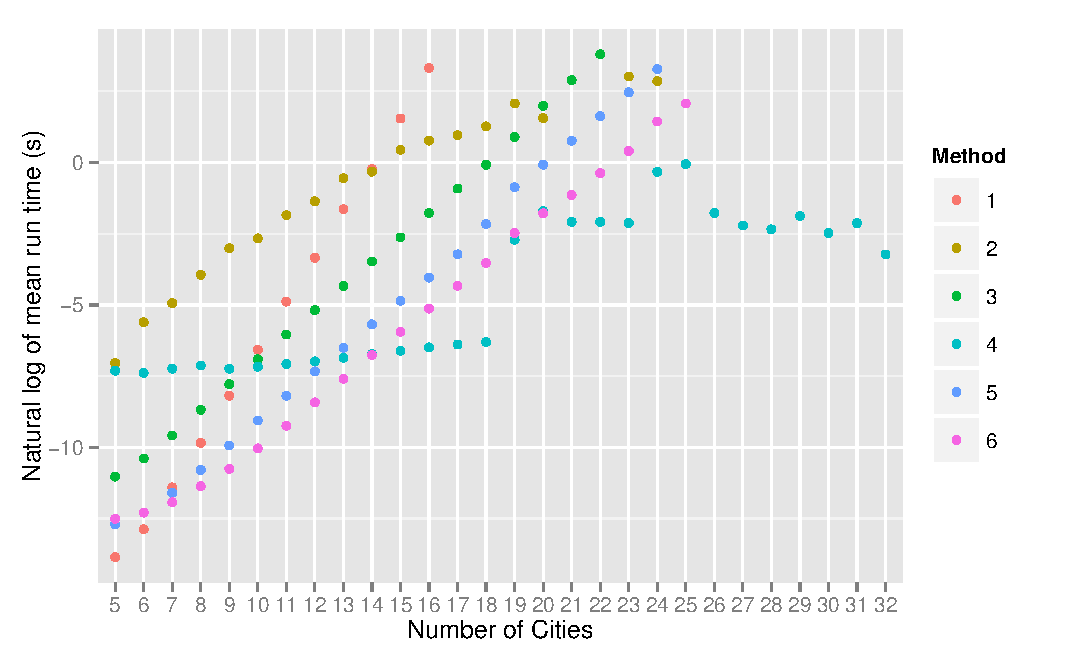
\includegraphics[width=0.8\textwidth]{s1-log}
		\caption{Mean running times of various algorithms on different sized geometric TSP problems. Computed on machine 1.}
		\label{fig:m1-runtime}
	\end{figure}
	
	\begin{figure}[H]
		\center
		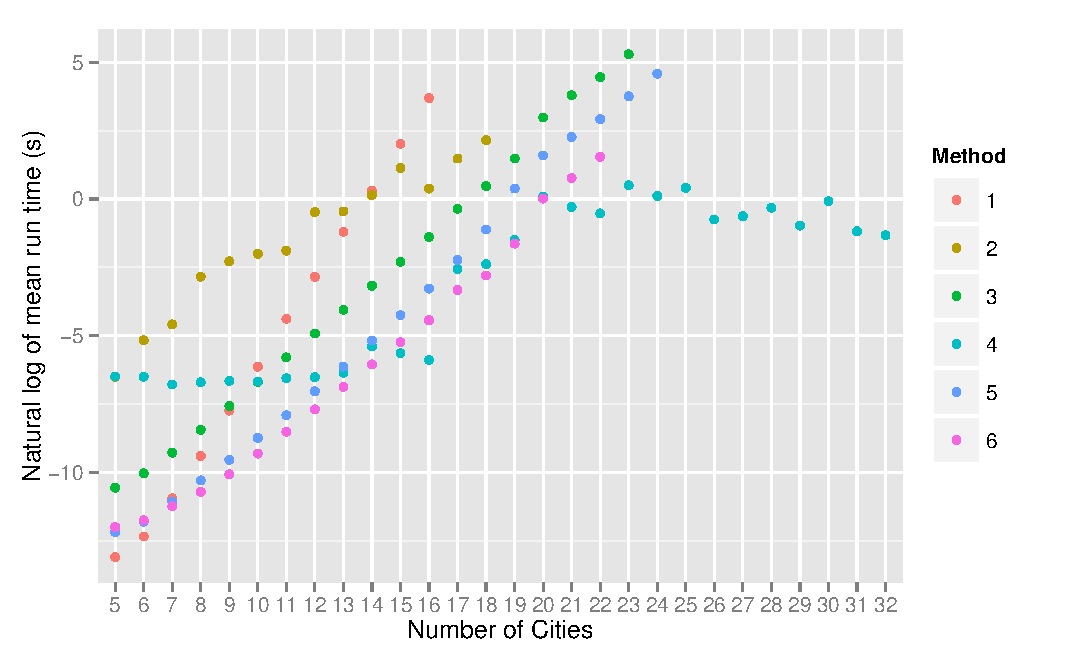
\includegraphics[width=0.8\textwidth]{b40-log}
		\caption{Mean running times of various algorithms on different sized geometric TSP problems. Computed on machine 2.}
		\label{fig:m2-runtime}
	\end{figure}
	
	Figure~\ref{fig:perf-5} shows that for n=5, enumeration has the most wins. It is always the best algorithm. Branch and cut is within a factor 1000 of the best algorithm, and BHK is about a factor 3 of the best algorithm. The 1-Tree algorithm solves 70\% of the problems in a factor of 1000 of the best algorithm. 

	\begin{figure}[H]
		\center
		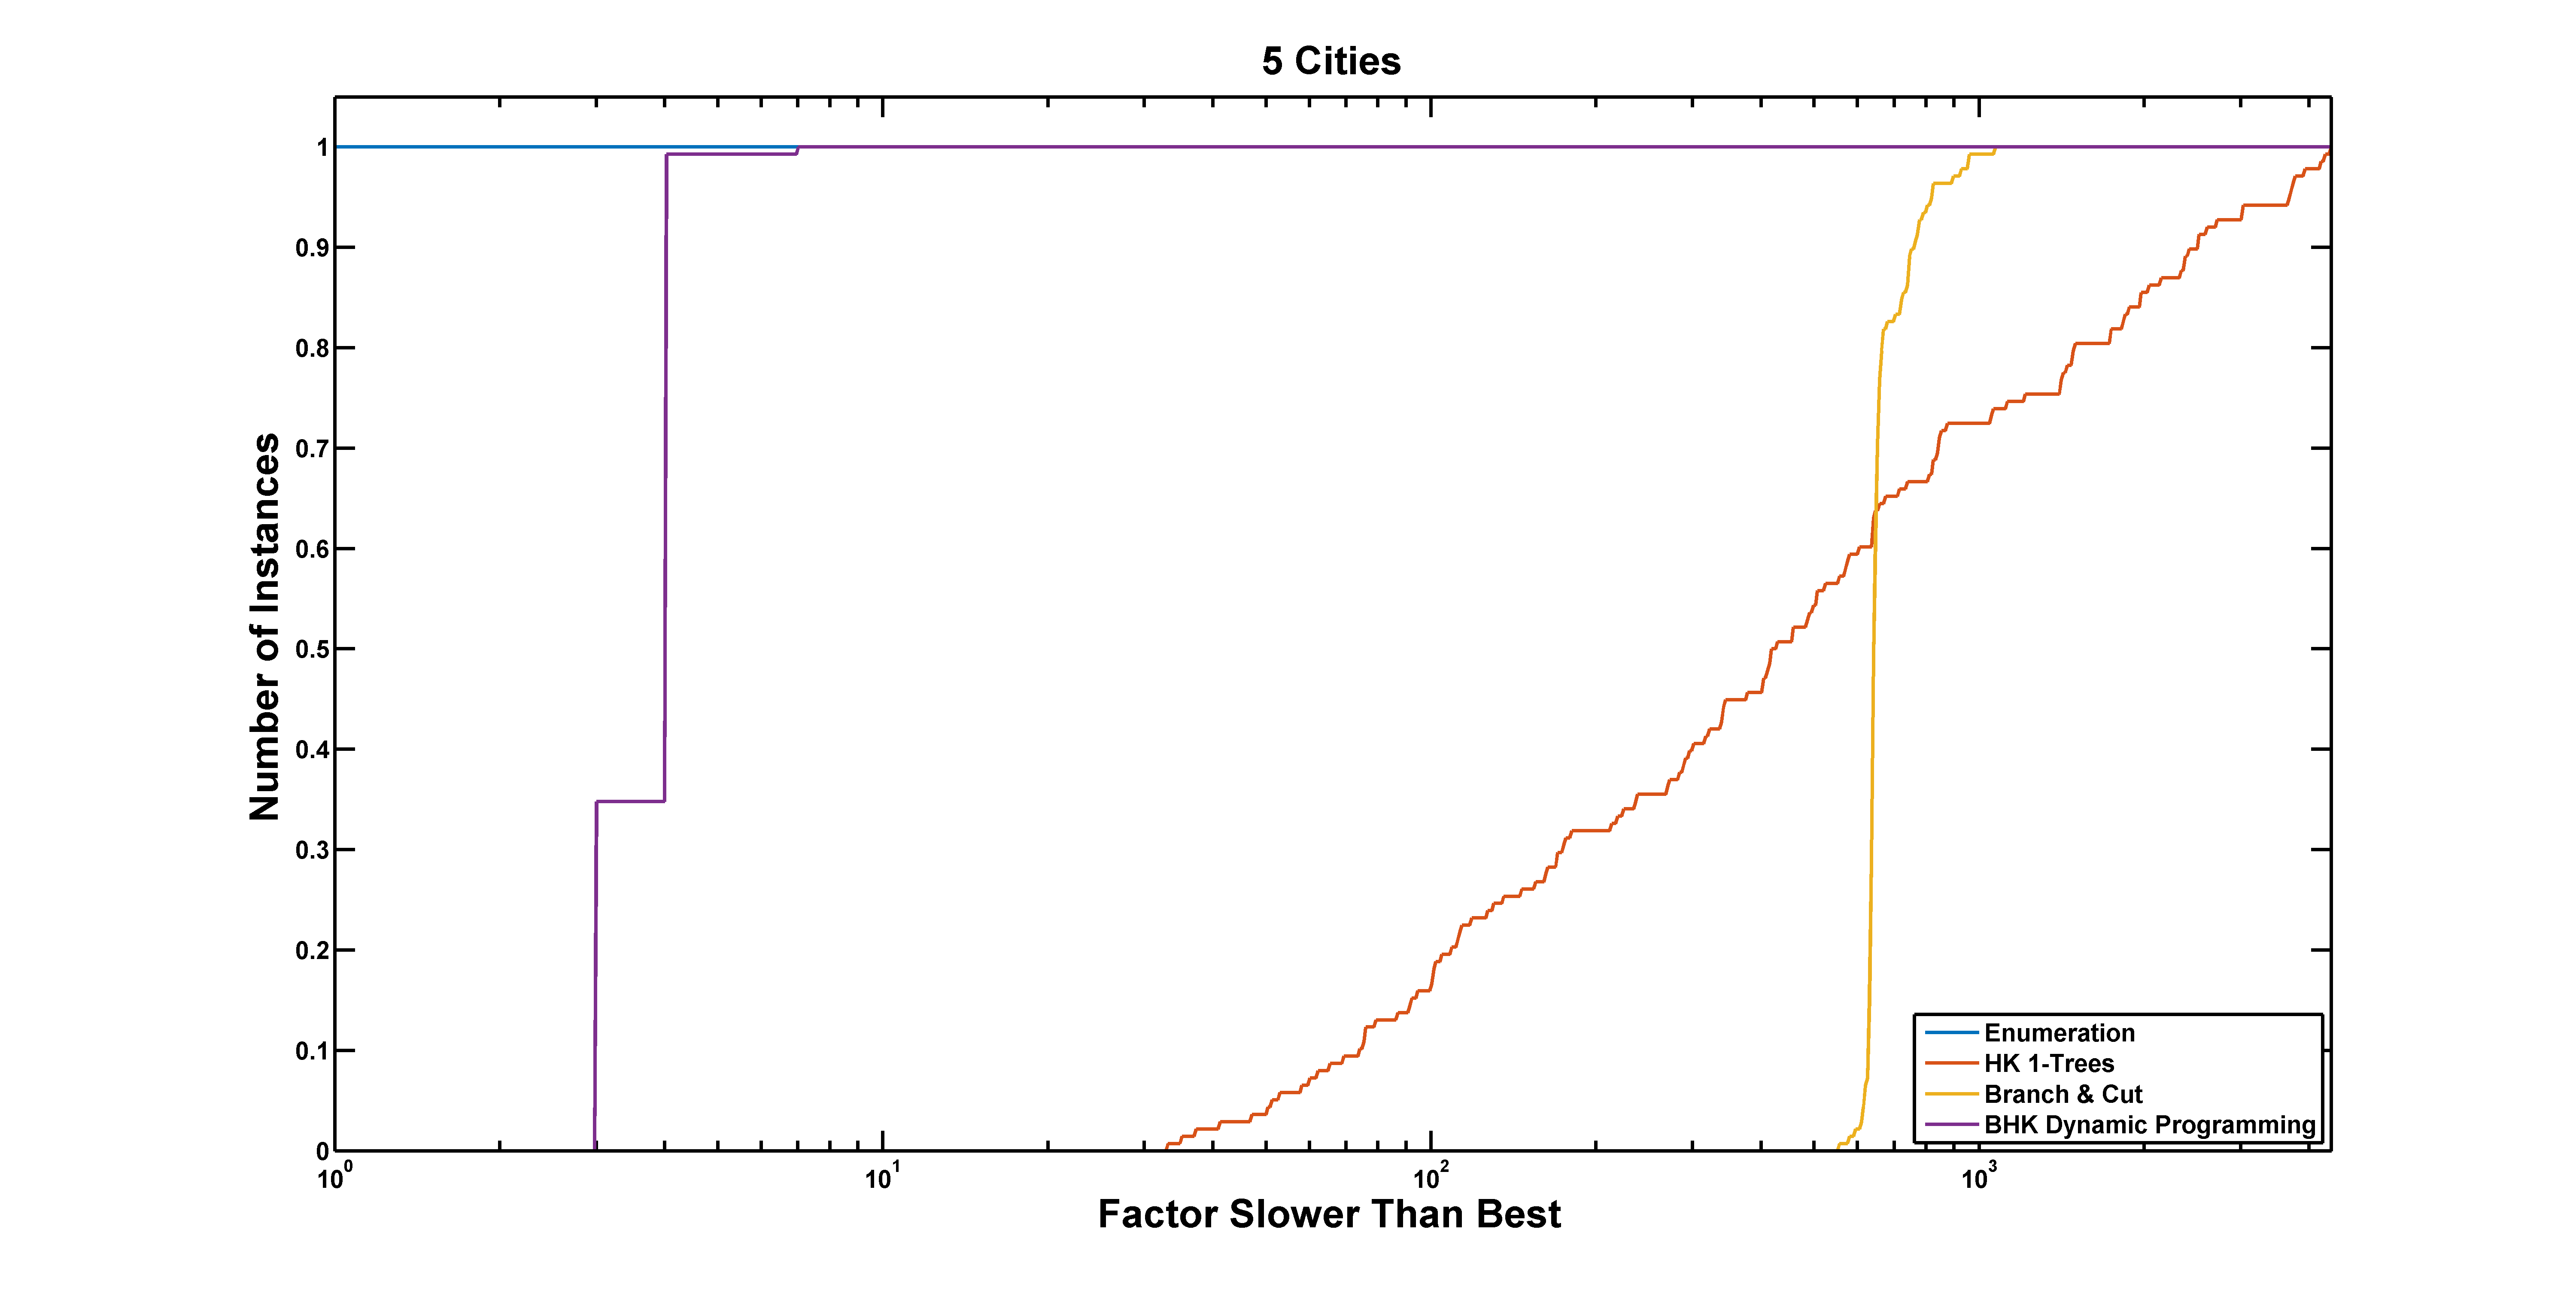
\includegraphics[width=0.95\textwidth]{../performanceplots/perf5_norm.png}
		\caption{Performance profiles of algorithms on instances of size 5.}
		\label{fig:perf-5}
	\end{figure}
	
	Figure~\ref{fig:perf-10} shows that for n=10, enumeration and branch and cut are on par solving within a factor 200 of the best algorithm. However, BHK dynamic programming is the overall winner. 
		
	\begin{figure}[H]
		\center
		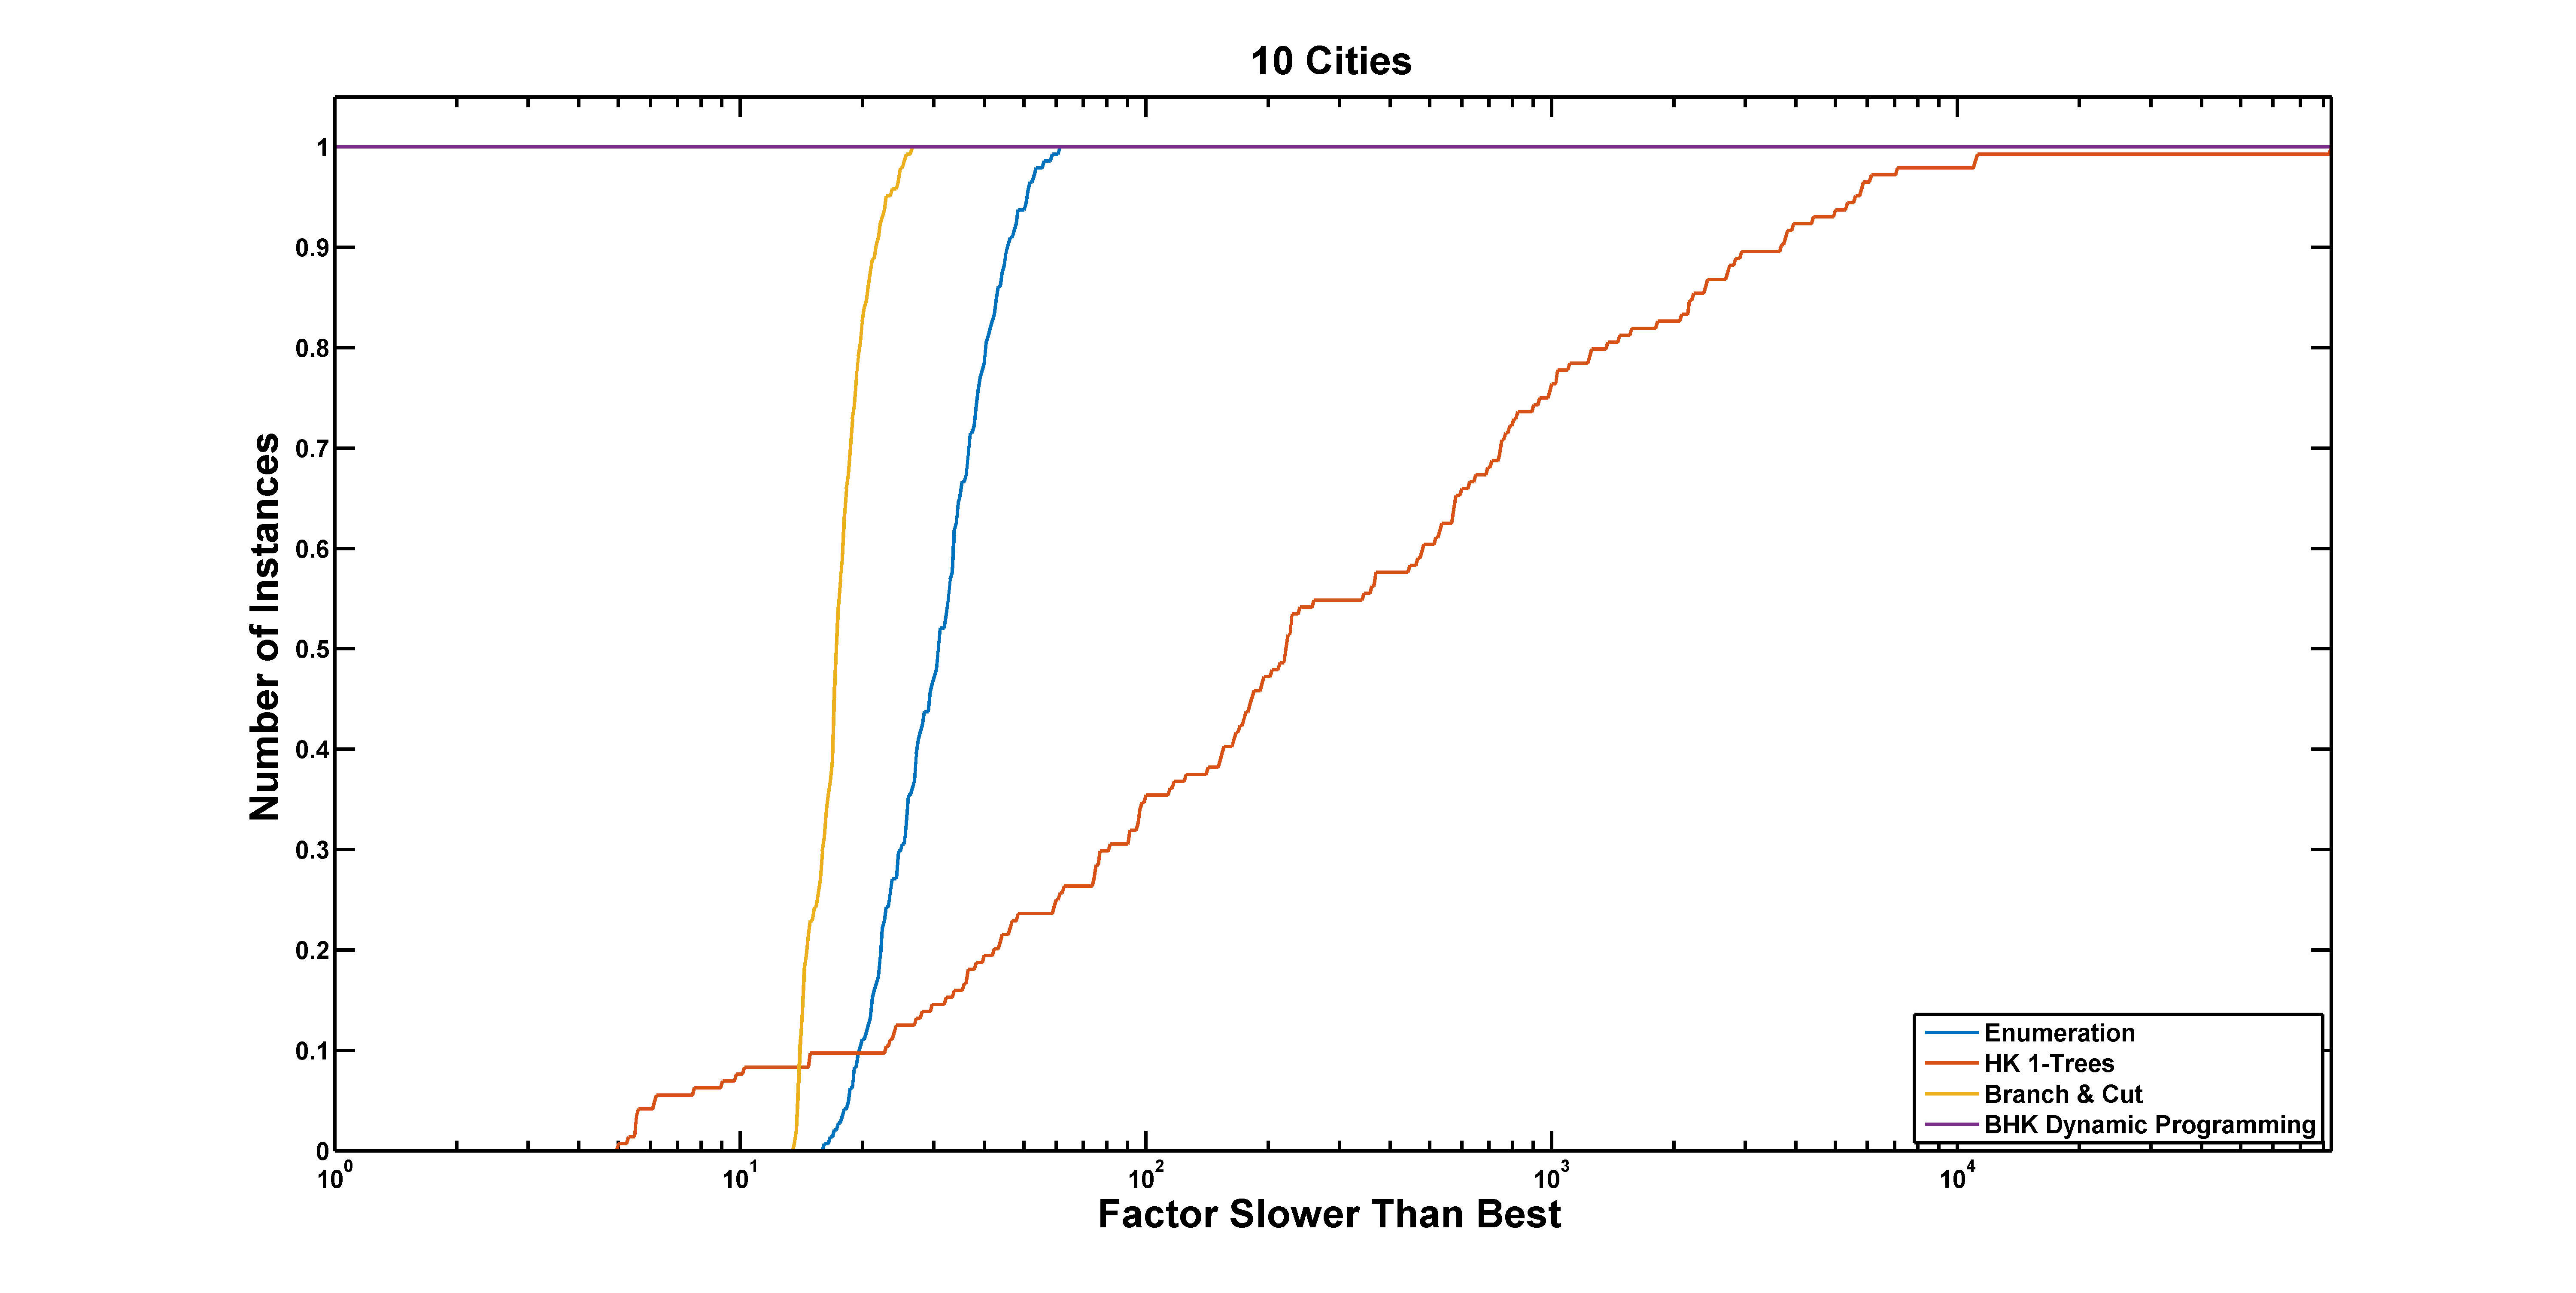
\includegraphics[width=0.95\textwidth]{../performanceplots/perf10_norm.png}
		\caption{Performance profiles of algorithms on instances of size 10.}
		\label{fig:perf-10}
	\end{figure}
	
	Finally, for n=15 branch and cut becomes has the most wins. The probability that it is the best algorithm is about .98. BHK dynamic programming is a factor of 2 slower than the best for 90\% of the problems as show in Figure~\ref{fig:perf-15}. 
	
	\begin{figure}[H]
		\center
		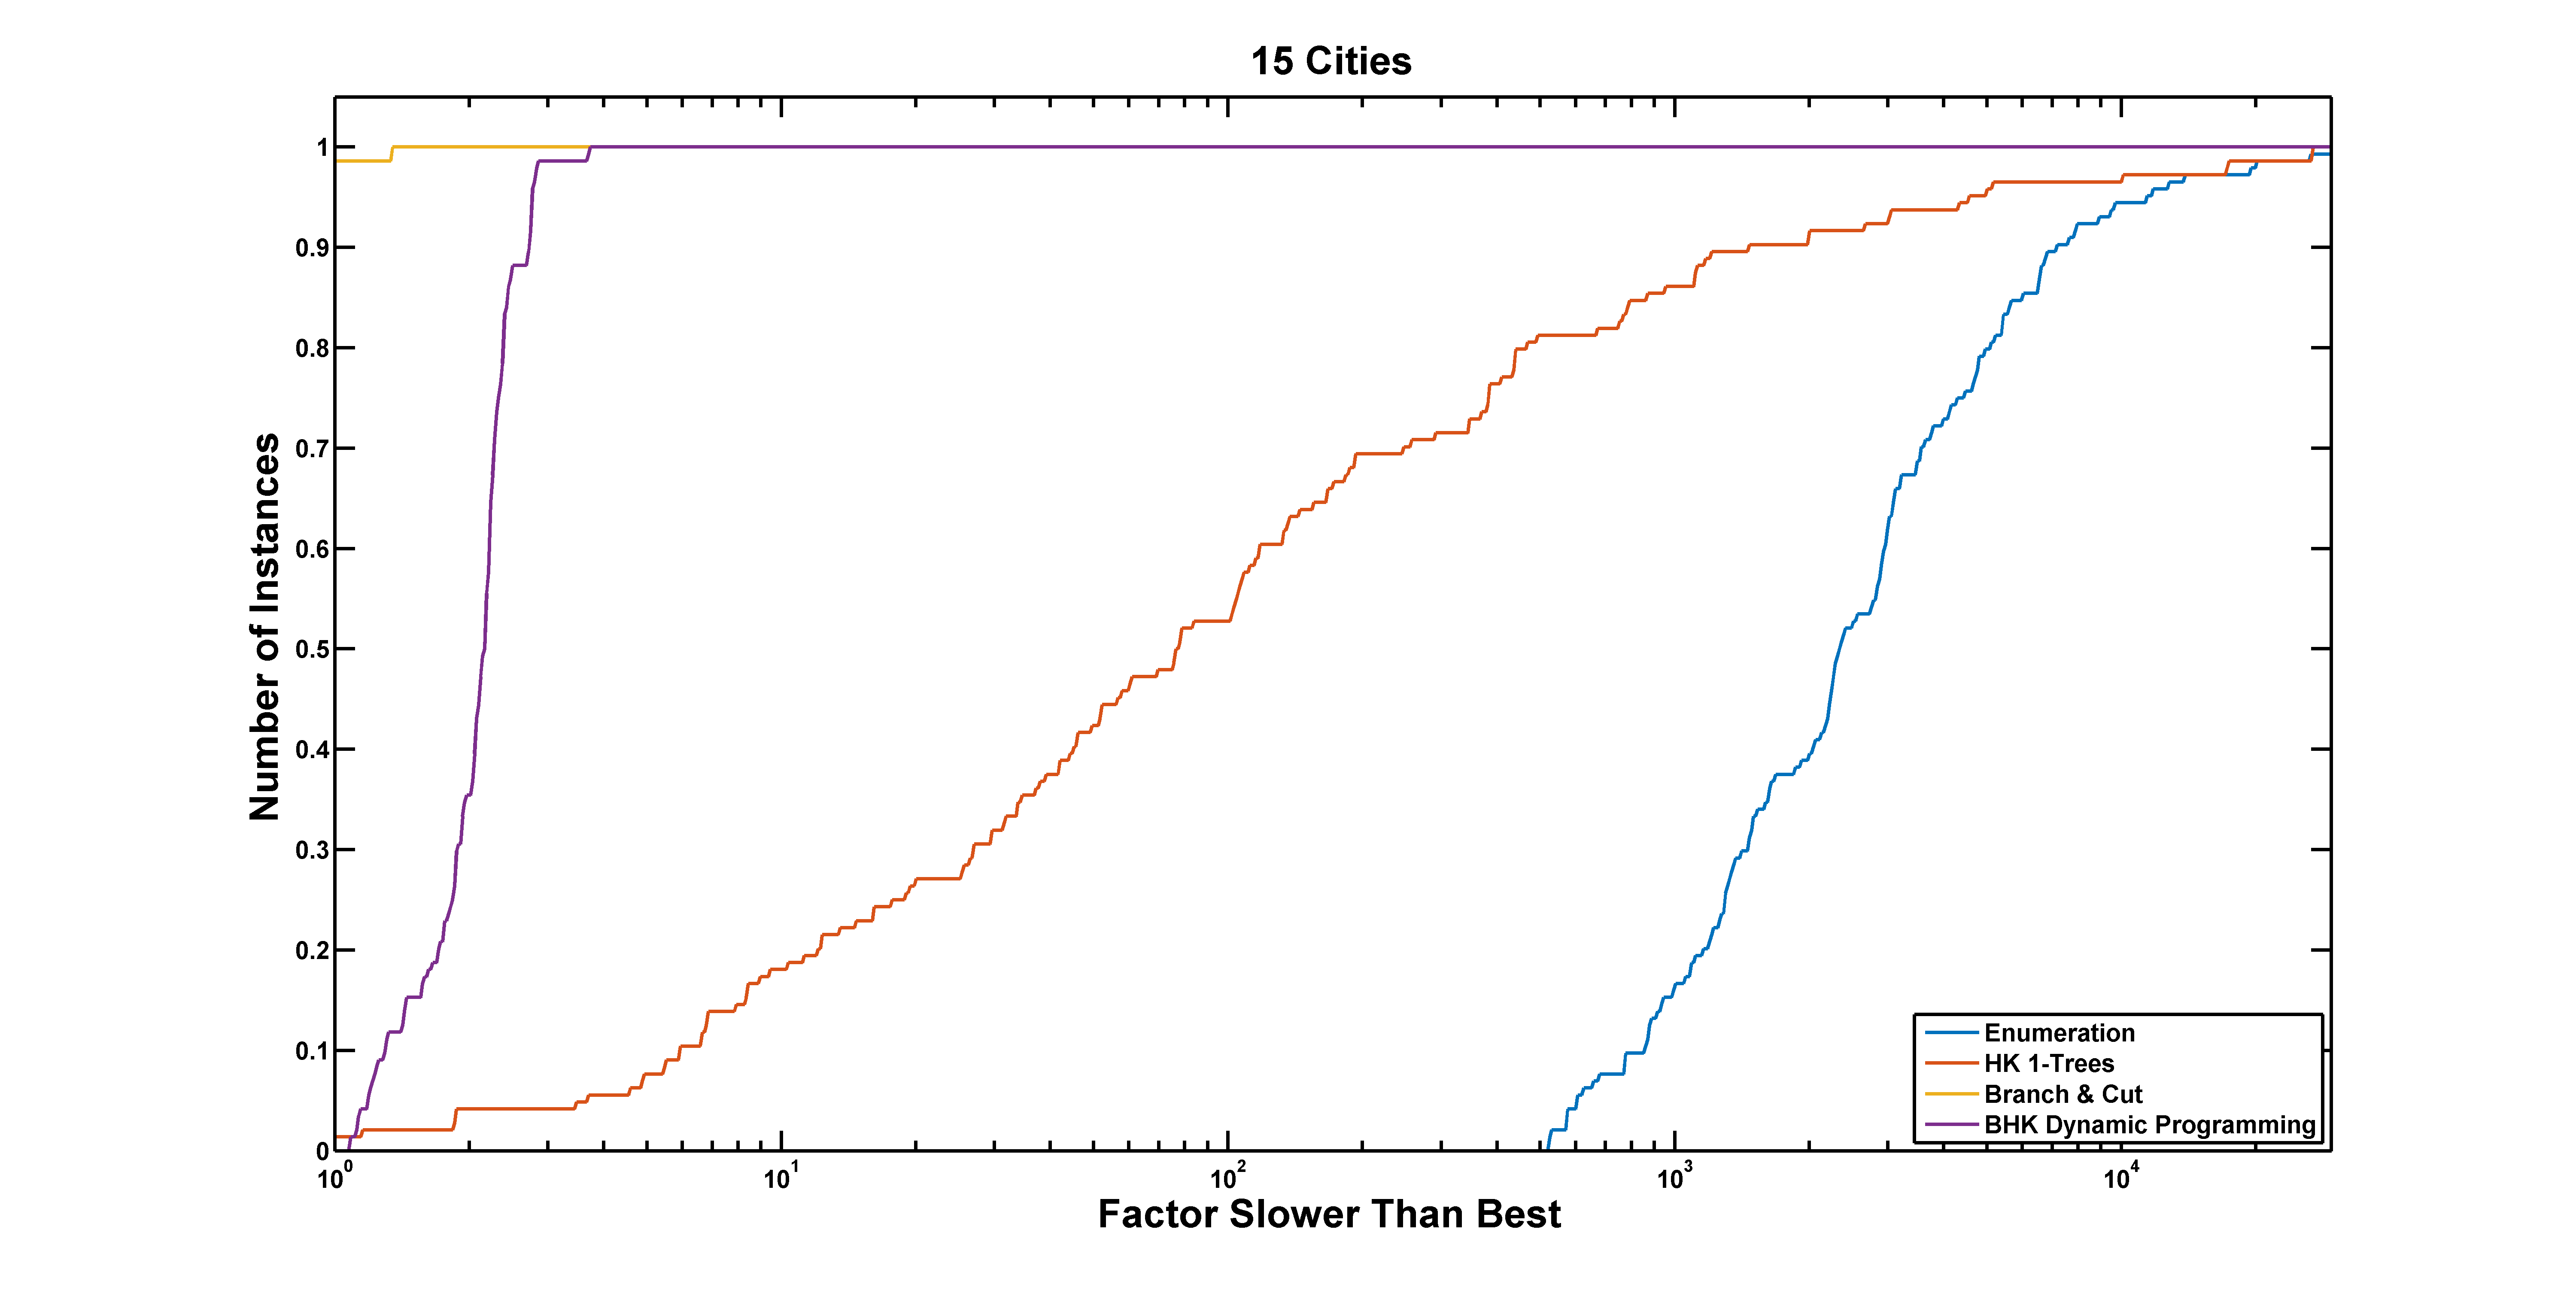
\includegraphics[width=0.95\textwidth]{../performanceplots/perf15_norm.png}
		\caption{Performance profiles of algorithms on instances of size 15.}
		\label{fig:perf-15}
	\end{figure}
	\section{Future Work}
	\label{sec:future}
	After a careful analysis of the data collected from experiments, we found that several seed and grid sizes were repeated in our experiment. This is due to the fact that the random numbers were generated between 1 and 100. For future experiments, we would like to ensure that no two random seeds are the same in our experiment. 
	
	In addition, for an ideal experiment design we would like to randomly assign grid sizes and city sizes during the experiment rather than iterating through them in order. Iterating through them in order may in fact be causing extra disk swapping. Once some algorithms reach n=20, they may consume more memory than the available physical RAM. Therefore, they may time out due to previous experiment runs that were swapping memory to disk. 
	
	\section{Conclusions}
	\label{sec:conclusions}
	For this project, we implemented four algorithms for solving the TSP and collected experimental results of their run times. The experimental data shows that the instance size, method, and seed have a significant effect on run times. As the number of cities increases from 5 to 25, enumeration is the best, succeeded by BHK dynamic programming, followed by branch and bound linear programming. Our performance profiles illustrate that these algorithms are the clear cut winner for 5, 10, and 15 cities. 
	
	
	\nocite{*}
	\bibliographystyle{plain}
	\bibliography{references}
	
	\section*{Appendix}
	\subsection*{Result Tables}
	\subsection*{Code}
	Relevant code files are as follows:
	
	\begin{itemize}
		\item Main program driver, Nearest-Neighbour, Branch-Cut code: \texttt{tour.cpp}
		\item Graph constructs: \texttt{graph.cpp, edge.cpp, tnode.cpp}
		\item 1-Tree Code: \texttt{onetree.cpp}
		\item BHK Dynamic Programming: \texttt{bhk1.cpp, bhk2.cpp, bhk3.cpp}
		\item Datamill scripts: \texttt{collect.sh, run.sh, setup.sh, tour.sh}
	\end{itemize}
	
	
	%%%%%%%%%%%%%%%%%%%%%%%%%%%%%%%%%%%%%%%%%%%%%%%%%%%%%%%%%
	
\end{document}